% \begin{document}

\usetikzlibrary{arrows.meta} % For double arrows

\chapter{Decentralized Database}

In the era of big-data today, localized instance of relational database is no
longer enough to hold the volume of data for toady's requirement. Distributed
key-value store has been of a key area of interest in the past few decades. 
Offering such as DynamoDB, Cassandra, Azure Cloud are a few examples of what
industry leaders are offering to address the data problem.\\

Service provided by a distributed key-value store is collectively offered by a
cluster of nodes. The nodes independently restart, update, crash, join or leave 
the cluster, while the service remains uninterrupted (though with possibly
reduced service). As the user base scales, the service must scale accordingly.\\

Two of the key design principles in a distributed data are partition and
replication.\\

A replica group (RG) is a group of nodes that maintain the same set of data.
Nodes in a RG often spans multiple availability zone (AZ) to maximize uptime.
In case of a regional value that wipes out an entire AZ, the other nodes in the
RG can still maintain the service albeit at reduced QoS. The nodes in the RG are
kept in sync using consensus protocol such as Raft. Typically, a write is only
considered complete and ack'd to client once it has been recorded by the
majority of nodes in the RG.

Partition is a way to split the keyspace into slices. When the keyspace is
partitioned, a RG is only responsible for a slice of the keyspace. Bandwidth
demand is also amortized across all RGs. Partition is typically done using 
consistent hashing. Different from traditional hashing, consistent hashing
minimizes data movement when nodes join and leave the clusters. Consistent
hashing will be covered in detail in a later part of the chapter.\\

Some of the early distributed database design requires a centralized server for
meta management (eg. ZooKeeper). In this chapter, we will specify a fully
decentralized key-value store. To simplify the specification, we will assume 
each node itself is a functioning RG with associated reliability property (this
is considered a solved problem with Raft).This chapter will focus on system
behavior correctness as RGs join or leave the cluster and associated data
migration.

\section{Consistent Hashing}

Before we dive into design detail, we must first describe consistent hashing.
With a traditional hashing algorithm, changing the size of the hash space
requires data movement of the entire cluster. This is very undesirable.
Consistent hashing was introduced to minimize data movement, where movement is
only required when adding or removing nodes in the affected range. 

In consistent hashing, the hash space is assumed to be a ring, where the largest
hash value plus one wraps around to the hash of 0. Servers in a consistent
hashing cluster take up different ranges in the ring. For a given request, the
client where the request lands by hashing the request first, then walks the ring
clockwise until it finds a server. \\ 

Assume the following example:

\begin{center}
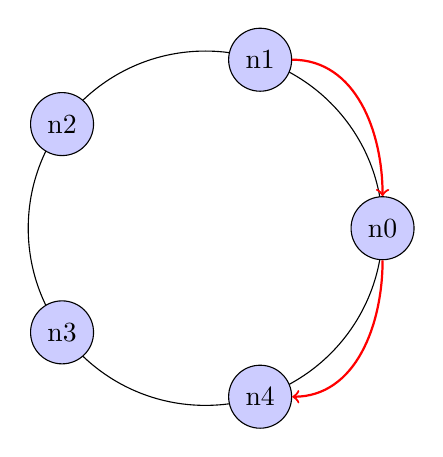
\begin{tikzpicture}[scale=1.5]

    \draw (0,0) circle (1.5cm);

    Draw the nodes on the circle with updated labels
    \foreach \angle/\label in {0/n0, 72/n1, 144/n2, 216/n3, 288/n4} {
        \node[draw, circle, fill=blue!20, minimum size=8mm] at (\angle:1.5cm) (\label) {\label};
    }

    \draw[->, thick, red] (n1) to[out=0, in=90] (n0); % 2 -> 1
    \draw[->, thick, red] (n0) to[out=270, in=0] (n4); % 1 -> 5

\end{tikzpicture}
\end{center}

If the request lands between n1 (exclusive) and n0 (inclusive), the request will
be processed by n0. Similarly, if the request lands between n0 (exclusive) and
n4 (inclusive), the request is to be processed by n4.\\

Assume a case where n4 goes offline: 

\begin{center}
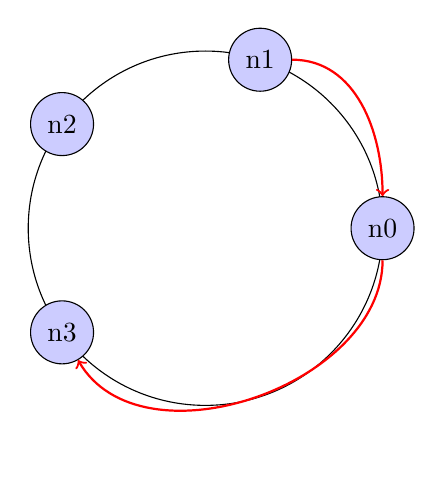
\begin{tikzpicture}[scale=1.5]

    \draw (0,0) circle (1.5cm);

    % Draw the nodes on the circle with updated labels
    \foreach \angle/\label in {0/n0, 72/n1, 144/n2, 216/n3} {
        \node[draw, circle, fill=blue!20, minimum size=8mm] at (\angle:1.5cm) (\label) {\label};
    }

    \draw[->, thick, red] (n1) to[out=0, in=90] (n0); % 2 -> 1
    \draw[->, thick, red] (n0) to[out=270, in=300] (n3); % 1 -> 5

\end{tikzpicture}
\end{center}

In such a case, requests previously processed by n4 will land on n3 instead.
Similarly, if a new node n5 is added:

\begin{center}
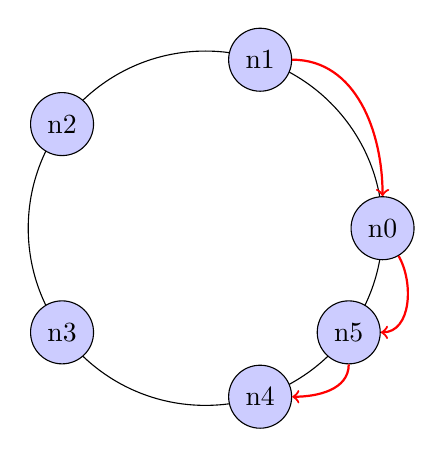
\begin{tikzpicture}[scale=1.5]

    % Draw the circle
    \draw (0,0) circle (1.5cm);

    % Draw the nodes on the circle with updated labels
    \foreach \angle/\label in {0/n0, 72/n1, 144/n2, 216/n3, 288/n4, 324/n5} {
        \node[draw, circle, fill=blue!20, minimum size=8mm] at (\angle:1.5cm) (\label) {\label};
    }

    % Draw arrows
    \draw[->, thick, red] (n1) to[out=0, in=90] (n0); % n1 -> n0
    \draw[->, thick, red] (n0) to[out=300, in=0] (n5); % n0 -> n4
    \draw[->, thick, red] (n5) to[out=270, in=0] (n4); % n0 -> n4

\end{tikzpicture}
\end{center}

Part of what n4 used to service will now be serviced by n5.

\section{Gossip Protocol}

Without a centralized metadata controller, the nodes learn about the peers using
gossip protocol. As a new RG enters the cluster, the design relies on gossip
protocol to spread the information. This is a critical part of the design as
will be described later.

\section{Design}

In our design, a RG can be in one of the following states: Offline, Joining,
Online, Leaving. The service starts with a single RG responsible for the entire
hash space. Since this is the epoch RG, it directly transitions into Online
state and can claim any token on the ring. For simplicity, epoch RG always claim
token 0.\\

The design assumes node failure handling are handled within the RG, the
specification will not model RG crash or restart. 

\subsection{Offline}

RG is offline, no impact to cluster.

\subsection{Joining}

By definition, the goal of adding a RG U into the cluster is to reduce the load
on another RG V. Since RG U is a new member of the cluster, it may not have the
latest cluster topology. Once RG U announces its presence via gossip protocol,
it waits for RG V to reach out.\\

When RG V realizes a new RG can share its burden, RG V will coordinate with RG U
to migrate a subset of its data to RG U (the subset RG U will be responsible
for). Once data migration completes: RG U transitions to Online state and start
servicing request in its range, while RG V rejects request to the range RG U has
taken over. This range update is also reflected in both RG U and V's local ring
cache, and communicated during next round of gossip protocol.

\subsection{Online}

RG is \textit{Online} and responds and records requests in its hash range. 

\subsection{Leaving}

Symmetrically, when a RG U is leaving the cluster, a RG V needs to take over the
range and data RG U is currently responsible for. Similarly to join, RG U 
announce its intent to leave, and wait for RG V to reach out and coordinate the
hand off.\\

Note when RG U is still waiting or in the middle of hand-off, it is still
\textit{Online} and must respond to request, until RV V fully takes over.

% Note this is a \textit{graceful} hand-off. The design assumes any failure
% mitigation is implemented within the RG. 


% Since the entire hash space is always covered by the cluster, a RG U joining 
% the cluster needs to coordinate with another RG V to take over part of RG V's 
% hash space. 
% take over a certain hash range needs to coordinate with RG V which is currently 
% responsible for that 
% cluster needs to coordinate with RG V that is currently responsible for the
% range. When RG U joins the cluster, it will announce its presence via gossip
% protocol. Eventually RG V will realize it can volunteer a part of its range to
% RG U, and 


% In this chapter, we will implement a simple distributed key-value store that
% supports horizontal scale-out. The service provider can add servers into the
% cluster dynamically to reduce the load on individual servers. Similarly, the
% service provider can also remove servers dynamically during off hours to
% minimize server costs.\\

% A new server \textit{K} joining the cluster claims a token \textit{T} on the
% ring. Starting from \textit{T}, walk the ring counter-clockwise to find the
% first neighboring token \textit{P}, \textit{K} owns the range of keys from
% \textit{P} (exclusive) to \textit{T} (inclusive).\\

% The design does not include replication or fault recovery to limit the scope.

\section{Specification}

The distributed key-value \textit{Init} is defined below:\\

\begin{tla}
offline == [k \in NodeState |-> 
            IF k = "version" THEN 0 
            ELSE IF k = "token" THEN -1
            ELSE IF k = "status" THEN "offline"
            ELSE "unused"]
seed == [k \in NodeState |-> 
            IF k = "version" THEN 1 
            ELSE IF k = "token" THEN 0
            ELSE IF k = "status" THEN "online"
            ELSE "unused"]

Init ==
    /\ cluster = {"n0"}
    /\ local_ring = [i \in Nodes |-> 
                        [j \in Nodes |-> 
                            IF i = "n0" /\ j = "n0" 
                            THEN seed
                            ELSE offline ]] 
    /\ local_kv = [i \in Nodes |-> {}]
    /\ debug_kv = {}
    /\ d1 = {}
\end{tla}
\begin{tlatex}
\@x{ offline \.{\defeq} [ k \.{\in} NodeState \.{\mapsto}}%
\@x{ {\IF} k \.{=}\@w{version} \.{\THEN} 0}%
\@x{ \.{\ELSE} {\IF} k \.{=}\@w{token} \.{\THEN} \.{-} 1}%
\@x{ \.{\ELSE} {\IF} k \.{=}\@w{status} \.{\THEN}\@w{offline}}%
\@x{ \.{\ELSE}\@w{unused} ]}%
\@x{ seed \.{\defeq} [ k \.{\in} NodeState \.{\mapsto}}%
\@x{\@s{4.1} {\IF} k \.{=}\@w{version} \.{\THEN} 1}%
\@x{\@s{4.1} \.{\ELSE} {\IF} k \.{=}\@w{token} \.{\THEN} 0}%
\@x{\@s{4.1} \.{\ELSE} {\IF} k \.{=}\@w{status} \.{\THEN}\@w{online}}%
\@x{\@s{4.1} \.{\ELSE}\@w{unused} ]}%
\@pvspace{8.0pt}%
\@x{ Init \.{\defeq}}%
\@x{\@s{16.4} \.{\land} cluster \.{=} \{\@w{n0} \}}%
\@x{\@s{16.4} \.{\land} local\_ring \.{=} [ i \.{\in} Nodes \.{\mapsto}}%
\@x{\@s{20.5} [ j \.{\in} Nodes \.{\mapsto}}%
\@x{\@s{24.6} {\IF} i \.{=}\@w{n0} \.{\land} j \.{=}\@w{n0}}%
\@x{\@s{24.6} \.{\THEN} seed}%
\@x{\@s{24.6} \.{\ELSE} offline ] ]}%
 \@x{\@s{16.4} \.{\land} local\_kv \.{=} [ i \.{\in} Nodes \.{\mapsto} \{ \}
 ]}%
\@x{\@s{16.4} \.{\land} debug\_kv \.{=} \{ \}}%
\@x{\@s{16.4} \.{\land} d1 \.{=} \{ \}}%
\end{tlatex}

\begin{itemize}
    \item \textit{cluster} is a set that includes all the nodes currently in the distributed key-value store.
    \item \textit{global\_ring} is a function that implements key-to-node mapping.
    \item \textit{local\_kv} represents the per node key-value store. For
    simplicity the key and value are assumed to be the same, thus represented
    as a single number.
    \item \textit{global\_kv} represents the system key-value store, used to check consistency.
\end{itemize}

Before we define the \textit{Spec}, we need create a few helper functions:\\
